\documentclass[two side,journal]{IEEEtran}
\usepackage{amsmath,amsfonts}
\usepackage{pgfplots}
\pgfplotsset{compat=1.6}
\usepackage{amssymb}
\usepackage{tikz}
\usepackage{tikzscale}
\usetikzlibrary{shapes,arrows,3d,positioning,calc,spy}
\usepackage{xcolor}

\begin{document}

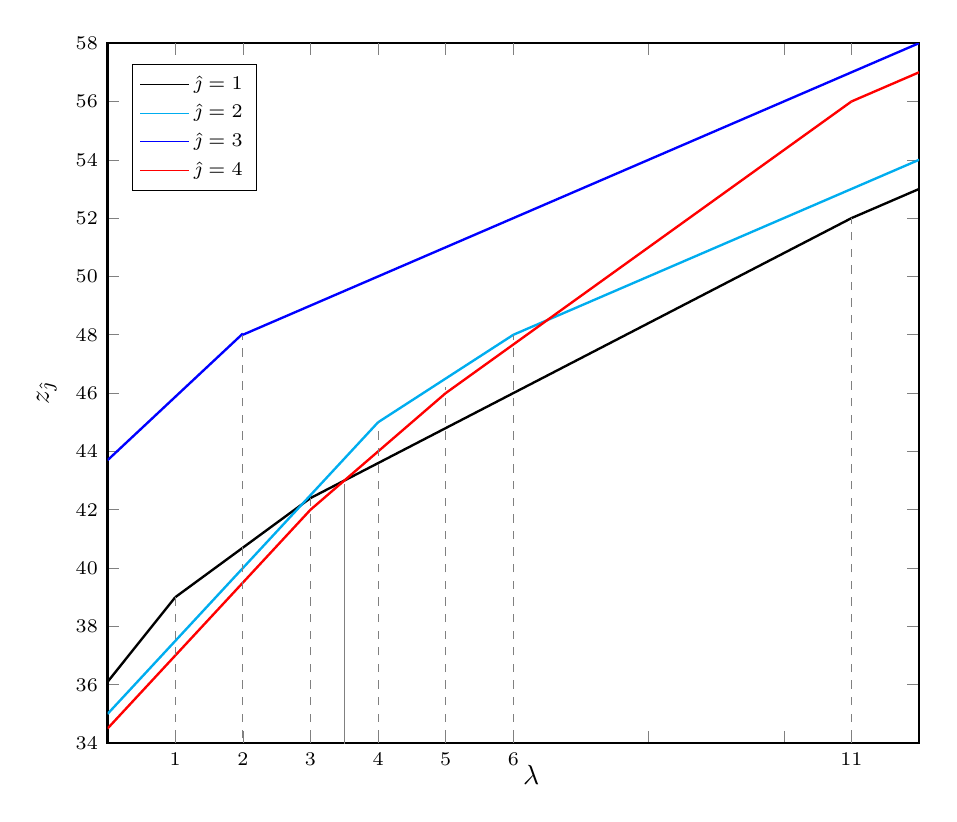
\begin{tikzpicture}  
\begin{axis}[%
    width=0.85\columnwidth,
    scale only axis,
    compat=newest,
    ylabel style = {align=left},
    axis line style=thick,
    inner axis line style={=>},
    xlabel={$\lambda$},  
    ylabel={$z_{\hat{\jmath}}$}, 
      x label style={anchor=west},
        y label style={anchor=south},
    ymin=34,ymax=58,
    legend pos=north west,
    xmin=0,xmax=12,
    xticklabels={},
    extra x ticks = {1,2,3,4,5,6,11},
    ticklabel style = {font=\scriptsize},
    legend style={font=\scriptsize},
    legend entries={$\hat{\jmath}=1$,
    $\hat{\jmath}=2$,
    $\hat{\jmath}=3$,
    $\hat{\jmath}=4$
    }
]
\addplot[line width=0mm ]{0};
\addplot[line width=0mm,cyan]{0}; 
\addplot[line width=0mm,blue]{0};  
\addplot[line width=0mm,color=red]{0};

\addplot[line width=0.3mm,domain=0:1 ]{36.1+2.9*x};
\addplot[line width=0.3mm,domain=1:3 ]{37.3+1.7*x}; 
\addplot[line width=0.3mm,domain=3:11 ]{38.8+1.2*x};  
\addplot[line width=0.3mm,domain=11:12 ]{41+1*x};

\addplot[line width=0.3mm,domain=0:4, cyan]{35+2.5*x};
\addplot[line width=0.3mm,domain=4:6, cyan,]{39+1.5*x};  
\addplot[line width=0.3mm,domain=6:12, cyan,]{42+1*x};  

\addplot[line width=0.3mm,domain=0:2, blue]{43.7+2.17*x};
\addplot[line width=0.3mm,domain=2:12, blue]{46+x}; 

\addplot[line width=0.3mm,domain=0:3,red,]{34.5+2.5*x};
\addplot[line width=0.3mm,domain=3:5,red,]{36+2*x};    
\addplot[line width=0.3mm,domain=5:11,red,]{37.66666+1.66666*x};
\addplot[line width=0.3mm,domain=11:12,red]{45+x};     

\draw[dashed,gray] (1,0) -- (1,39);
\draw[dashed,gray] (2,0) -- (2,48);
\draw[dashed,gray] (3,0) -- (3,42.4);
\draw[dashed,gray] (4,0) -- (4,45);
\draw[dashed,gray] (5,0) -- (5,46.2);
\draw[dashed,gray] (6,0) -- (6,48);
\draw[dashed,gray] (11,0) -- (11,52);

\draw[gray] (3.5,0) -- (3.5,42.9);
\end{axis}
\end{tikzpicture}

\end{document}